\section{Modularisierung}
\subsection{Motivation \buch{p.9}}
\begin{center}
{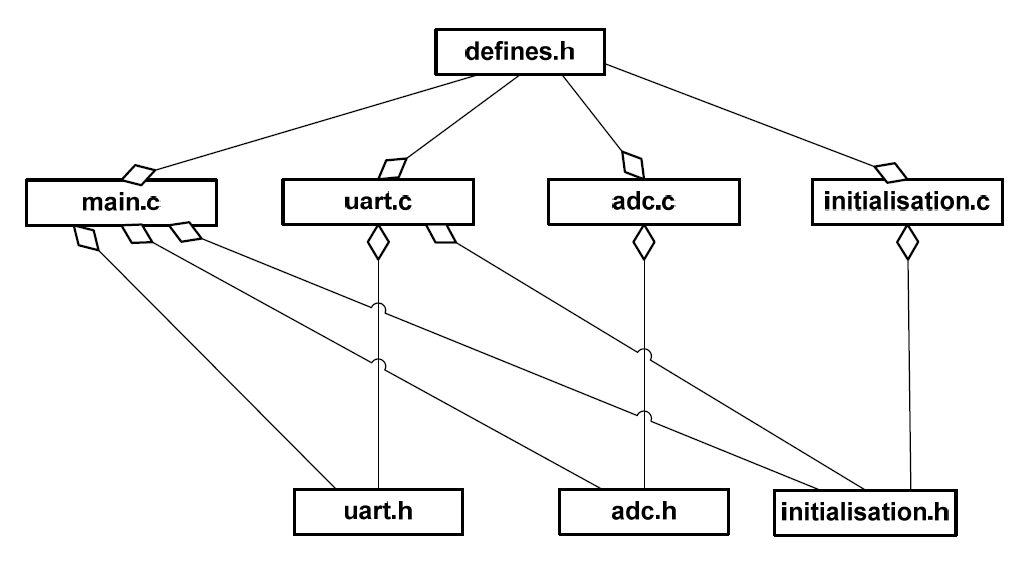
\includegraphics[width=0.5\textwidth]{images/Modularisierung/SchlechtesBeispielModularisierung.png}}
%\label{Fig: Schlechtes Beispiel für Modularisierung}
\end{center}
Bei Kleinstsoftware braucht es kein systematisches Design, da man diese meist
auch nicht ausbauen möchte. Vernünftige SW-Projekte will man jedoch meist noch
weiter ausbauen können.\\
Wichtig ist daher:\\
\begin{itemize}
  \item Schnittstellen definieren
  \item Modularisierung
\end {itemize}
\subsection{Grundprinzip}
\begin{itemize}
  \item Divide et impera
  \begin{itemize}
    \item Problem aufteilen in Unterprobleme, diese einzeln angehen
    \item Zuerst Grobentwurf, dann verfeinern (Top-Down-Prinzip)
  \end{itemize}
  \item \textbf{Ziel:} Reduktion der Komplexität
\end{itemize}
\subsection{Information Hiding}
\begin{itemize}
  \item Nutzer des Moduls braucht nur die Schnittstelle zu kennen (*.h files)
  \item Über inneren Aufbau dürfen keine Annahmen getroffen werden
  \item Der innere Aufbau (*.cpp files) muss nicht bekannt sein
\end{itemize}
\subsection{Hauptkriterien der Zerlegung}
\begin{itemize}
  \item Hauptkriterien
  \begin{itemize}
    \item Kopplung/Coupling
    \begin{itemize}
      \item Mass für Komplexität der Schnittstelle
    \end{itemize}
    \item Kohäsion/Cohesion
    \begin{itemize}
      \item Aussage wie stark eine funktionale Einheit wirklich zusammengehört
      \item Mass für die Stärke des inneren Zusammenhangs 
    \end{itemize}
  \end{itemize}
  \item \textbf{Ziel:} Schwache Kopplung, starke Kohäsion 
\end{itemize}
\begin{center}
{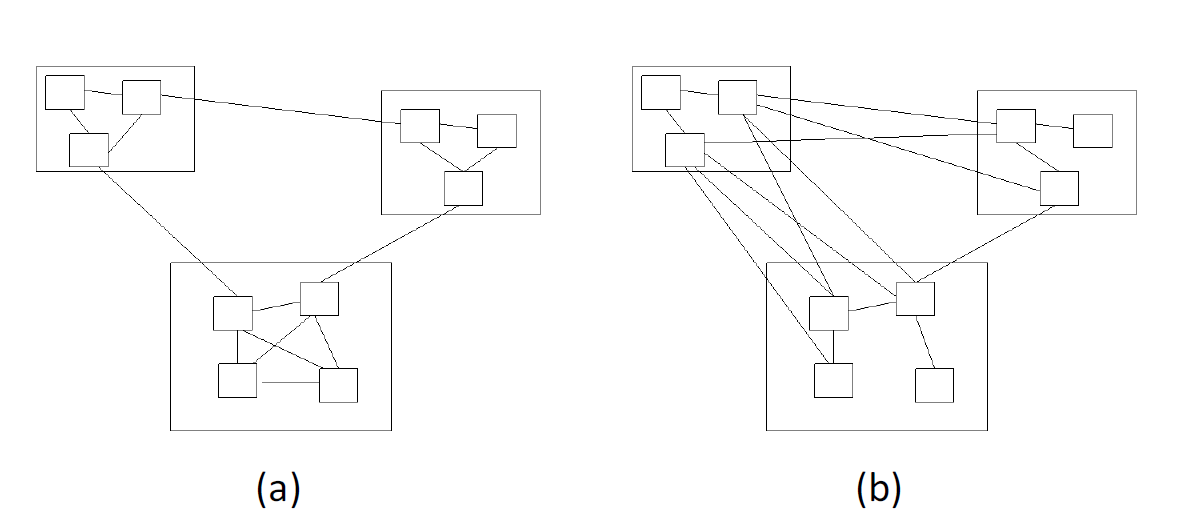
\includegraphics[width=0.5\textwidth]{images/Modularisierung/BeispieleKopplungKohaesion.png}}
%\label{Fig: Schlechtes Beispiel für Modularisierung}
\end{center}
\begin{itemize}
  \item Bild a: Hohe Kohäsion, niedrige Kopplung (gut)
  \item Bild b: Niedrige Kohäsion, hohe Kopplung (schlecht)
\end{itemize}
\subsection{Definitionen Kopplung}
\begin{itemize}
  \item Keine direkte Kopplung (Schwache Kopplung $\rightarrow$ \textbf{GUT})
  \item Datenkopplung
  \begin{itemize}
    \item Kommunikation ausschliesslich über Parameter 
  \end{itemize}
  \item Datenbereichskopplung
   \begin{itemize}
    \item Modul hat Zugriff auf Datenstruktur eines anderen Moduls
    \item Es werden nur einzelne Kompenenten benötigt
  \end{itemize}
  \item Steuerflusskopplung
  \begin{itemize}
    \item Modul beeinflusst Steuerfluss eines anderen Moduls
  \end{itemize}
  \item Globale Kopplung
  \begin{itemize}
    \item Kommunikation über globale Variabeln
    \item Jedes Modul hat Zugriff
  \end{itemize}
  \item Inhaltskopplung (Starke Kopplung $\rightarrow$ \textbf{SCHLECHT})
  \begin{itemize}
    \item Aus einem Modul werden lokale Daten eines anderen Moduls modifiziert,
    obwohl dieses Modul NICHT vom anderen Modul aufgerufen worden ist. 
    \item \textbf{Todsünde}
  \end{itemize}
\end{itemize}
\subsection{Definitionen Kohäsion}
\begin{itemize}
  \item Funktionale Kohäsion (Starke Kohäsion $\rightarrow$ \textbf{GUT})
  \begin{itemize}
    \item Teile einer Einheit bilden zusammen eine Funktion 
  \end{itemize}
  \item Sequentielle Kohäsion
   \begin{itemize}
    \item Teilfunktionen einer Einheit werden nacheinander ausgeführt
    \item Das Ergebnis einer Teilfunktion ist die Eingabe der nächsten
  \end{itemize}
  \item Kommunikative Kohäsion
  \begin{itemize}
    \item Teilfunktionen einer Einheit werden auf den gleichen Daten ausgeführt
    \item Reihenfolge spielt keine Rolle
  \end{itemize}
  \item Prozedurale Kohäsion
  \begin{itemize}
    \item Teilfunktionen werden nacheinander ausgeführt
    \item Sind über Steuerfluss verknüpft
  \end{itemize}
  \item Zeitliche Kohäsion
  \begin{itemize}
    \item Teile einer Einheit sind alle zu einer bestimmten auszuführen
  \end{itemize}
  \item Logische Kohäsion
  \begin{itemize}
    \item Teilfunktionen einer Einheit gehören zu einer Klasse
  \end{itemize}
  \item Zufällige Kohäsion (Schwache Kohäsion $\rightarrow$ \textbf{SCHLECHT})
  \begin{itemize}
    \item Teilfunktionen einer Einheit haben keinen sinnvollen Zusammenhang
  \end{itemize}
\end{itemize}
\begin{multicols}{2}
Bestimmung der Kohäsion:
\begin{center}
{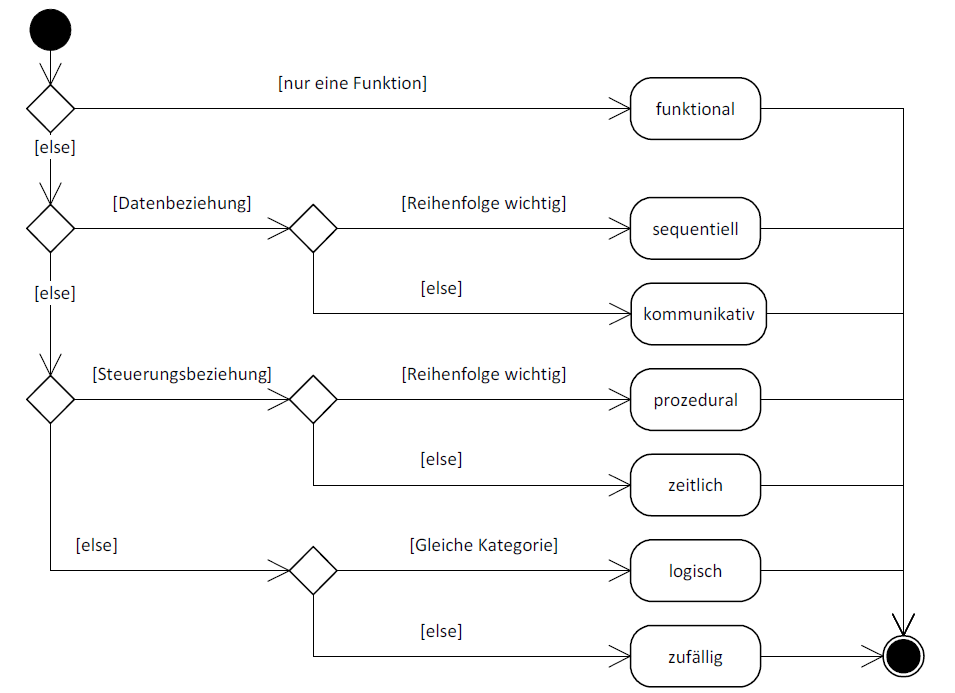
\includegraphics[width=0.5\textwidth]{images/Modularisierung/Kohaesionsbestimmung.png}}
%\label{Fig: Schlechtes Beispiel für Modularisierung}
\end{center}

\columnbreak

Ziele bezüglich Kohäsion
\begin{itemize}
  \item Kohäsion maximieren
  \item Idealerweise führt eine Unit nur eine Aufgabe (Funktion) aus
  \item Starke Kohäsion steigert
  \begin{itemize}
    \item Wartbarkeit
    \item Änderbarkeit
    \item Verständlichkeit
  \end{itemize}
  \item \textbf{Zusammengehörendes zusammen nehmen!}
  \item \textbf{Starke Kohäsion führt zu schwacher Kopplung, aber nicht umgekehrt!!}
\end{itemize}
\end{multicols}
\begin{center}
Beispiel guter Modularisierung:
{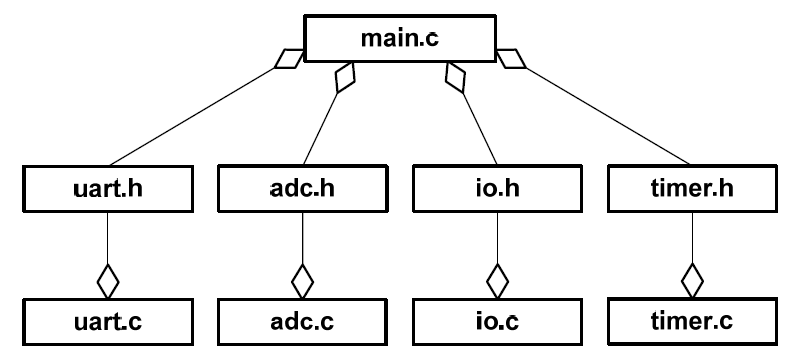
\includegraphics[width=0.5\textwidth]{images/Modularisierung/GutesBeispielModularisierung.png}}
%\label{Fig: Schlechtes Beispiel für Modularisierung}
\end{center}